\documentclass{standalone}
\usepackage{tikz}
\usetikzlibrary{patterns, positioning}


\begin{document}
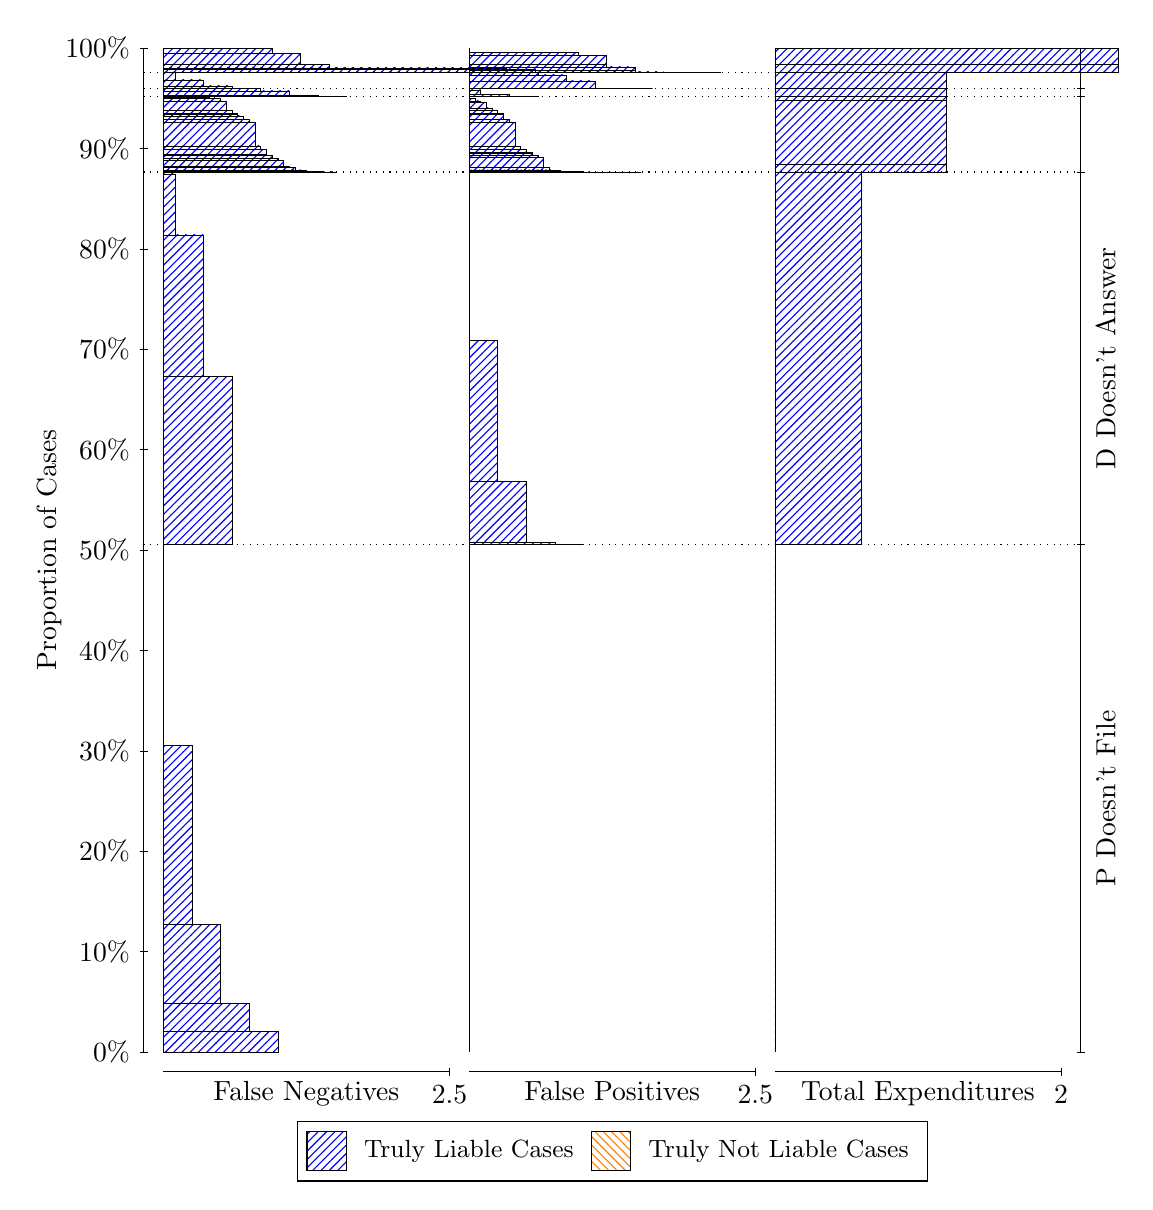
\begin{tikzpicture}
\draw[black, very thin] (1.5,1.75) -- (1.5,14.5);
\node[rotate=90, text=black, anchor=center] at (0.3, 8.125) {Proportion of Cases};
\draw[black, very thin] (1.45,1.75) -- (1.55,1.75);
\node[text=black, anchor=east] at (1.45, 1.75) {0\%};
\draw[black, very thin] (1.45,3.025) -- (1.55,3.025);
\node[text=black, anchor=east] at (1.45, 3.025) {10\%};
\draw[black, very thin] (1.45,4.3) -- (1.55,4.3);
\node[text=black, anchor=east] at (1.45, 4.3) {20\%};
\draw[black, very thin] (1.45,5.575) -- (1.55,5.575);
\node[text=black, anchor=east] at (1.45, 5.575) {30\%};
\draw[black, very thin] (1.45,6.85) -- (1.55,6.85);
\node[text=black, anchor=east] at (1.45, 6.85) {40\%};
\draw[black, very thin] (1.45,8.125) -- (1.55,8.125);
\node[text=black, anchor=east] at (1.45, 8.125) {50\%};
\draw[black, very thin] (1.45,9.4) -- (1.55,9.4);
\node[text=black, anchor=east] at (1.45, 9.4) {60\%};
\draw[black, very thin] (1.45,10.675) -- (1.55,10.675);
\node[text=black, anchor=east] at (1.45, 10.675) {70\%};
\draw[black, very thin] (1.45,11.95) -- (1.55,11.95);
\node[text=black, anchor=east] at (1.45, 11.95) {80\%};
\draw[black, very thin] (1.45,13.225) -- (1.55,13.225);
\node[text=black, anchor=east] at (1.45, 13.225) {90\%};
\draw[black, very thin] (1.45,14.5) -- (1.55,14.5);
\node[text=black, anchor=east] at (1.45, 14.5) {100\%};

\draw[black, very thin] (13.4,1.75) -- (13.4,14.5);
\draw[black, very thin] (13.35,1.75) -- (13.45,1.75);
\node[anchor=west] at (13.35, 1.75) {};
\draw[black, very thin] (13.35,8.1943) -- (13.45,8.1943);
\node[anchor=west] at (13.35, 8.1943) {};
\draw[black, very thin] (13.35,12.925) -- (13.45,12.925);
\node[anchor=west] at (13.35, 12.925) {};
\draw[black, very thin] (13.35,13.885) -- (13.45,13.885);
\node[anchor=west] at (13.35, 13.885) {};
\draw[black, very thin] (13.35,13.984) -- (13.45,13.984);
\node[anchor=west] at (13.35, 13.984) {};
\draw[black, very thin] (13.35,14.194) -- (13.45,14.194);
\node[anchor=west] at (13.35, 14.194) {};
\draw[black, very thin] (13.35,14.5) -- (13.45,14.5);
\node[anchor=west] at (13.35, 14.5) {};

\draw[black, very thin, pattern color=blue, pattern=north east lines] (1.75,1.75) rectangle (3.2033,2.0119);
\draw[black, very thin, pattern color=blue, pattern=north east lines] (1.75,2.0119) rectangle (2.84,2.3644);
\draw[black, very thin, pattern color=blue, pattern=north east lines] (1.75,2.3644) rectangle (2.4767,3.3722);
\draw[black, very thin, pattern color=blue, pattern=north east lines] (1.75,3.3722) rectangle (2.1133,5.647);
\draw[black, very thin, pattern color=orange, pattern=north west lines] (1.75,5.647) rectangle (1.75,5.647);
\draw[black, very thin, pattern color=blue, pattern=north east lines] (1.75,5.647) rectangle (1.75,8.1943);
\draw[black, very thin, pattern color=blue, pattern=north east lines] (1.75,8.1943) rectangle (2.622,10.333);
\draw[black, very thin, pattern color=blue, pattern=north east lines] (1.75,10.333) rectangle (2.2587,12.127);
\draw[black, very thin, pattern color=blue, pattern=north east lines] (1.75,12.127) rectangle (1.8953,12.902);
\draw[black, very thin, pattern color=orange, pattern=north west lines] (1.75,12.902) rectangle (1.75,12.902);
\draw[black, very thin, pattern color=blue, pattern=north east lines] (1.75,12.902) rectangle (1.75,12.925);
\draw[black, very thin, pattern color=blue, pattern=north east lines] (1.75,12.925) rectangle (3.93,12.927);
\draw[black, very thin, pattern color=blue, pattern=north east lines] (1.75,12.927) rectangle (3.7847,12.93);
\draw[black, very thin, pattern color=blue, pattern=north east lines] (1.75,12.93) rectangle (3.6393,12.936);
\draw[black, very thin, pattern color=blue, pattern=north east lines] (1.75,12.936) rectangle (3.5667,12.948);
\draw[black, very thin, pattern color=blue, pattern=north east lines] (1.75,12.948) rectangle (3.494,12.953);
\draw[black, very thin, pattern color=blue, pattern=north east lines] (1.75,12.953) rectangle (3.4213,12.982);
\draw[black, very thin, pattern color=blue, pattern=north east lines] (1.75,12.982) rectangle (3.3487,12.997);
\draw[black, very thin, pattern color=blue, pattern=north east lines] (1.75,12.997) rectangle (3.276,13.071);
\draw[black, very thin, pattern color=blue, pattern=north east lines] (1.75,13.071) rectangle (3.2033,13.1);
\draw[black, very thin, pattern color=blue, pattern=north east lines] (1.75,13.1) rectangle (3.1307,13.139);
\draw[black, very thin, pattern color=blue, pattern=north east lines] (1.75,13.139) rectangle (3.058,13.153);
\draw[black, very thin, pattern color=blue, pattern=north east lines] (1.75,13.153) rectangle (3.058,13.214);
\draw[black, very thin, pattern color=blue, pattern=north east lines] (1.75,13.214) rectangle (2.9853,13.257);
\draw[black, very thin, pattern color=blue, pattern=north east lines] (1.75,13.257) rectangle (2.9127,13.556);
\draw[black, very thin, pattern color=blue, pattern=north east lines] (1.75,13.556) rectangle (2.9127,13.561);
\draw[black, very thin, pattern color=blue, pattern=north east lines] (1.75,13.561) rectangle (2.84,13.596);
\draw[black, very thin, pattern color=blue, pattern=north east lines] (1.75,13.596) rectangle (2.7673,13.637);
\draw[black, very thin, pattern color=blue, pattern=north east lines] (1.75,13.637) rectangle (2.6947,13.653);
\draw[black, very thin, pattern color=blue, pattern=north east lines] (1.75,13.653) rectangle (2.6947,13.67);
\draw[black, very thin, pattern color=blue, pattern=north east lines] (1.75,13.67) rectangle (2.622,13.704);
\draw[black, very thin, pattern color=blue, pattern=north east lines] (1.75,13.704) rectangle (2.5493,13.824);
\draw[black, very thin, pattern color=blue, pattern=north east lines] (1.75,13.824) rectangle (2.5493,13.83);
\draw[black, very thin, pattern color=blue, pattern=north east lines] (1.75,13.83) rectangle (2.4767,13.858);
\draw[black, very thin, pattern color=blue, pattern=north east lines] (1.75,13.858) rectangle (2.404,13.858);
\draw[black, very thin, pattern color=blue, pattern=north east lines] (1.75,13.858) rectangle (2.404,13.866);
\draw[black, very thin, pattern color=blue, pattern=north east lines] (1.75,13.866) rectangle (2.3313,13.874);
\draw[black, very thin, pattern color=blue, pattern=north east lines] (1.75,13.874) rectangle (2.3313,13.874);
\draw[black, very thin, pattern color=blue, pattern=north east lines] (1.75,13.874) rectangle (2.2587,13.875);
\draw[black, very thin, pattern color=blue, pattern=north east lines] (1.75,13.875) rectangle (2.186,13.877);
\draw[black, very thin, pattern color=blue, pattern=north east lines] (1.75,13.877) rectangle (2.186,13.88);
\draw[black, very thin, pattern color=blue, pattern=north east lines] (1.75,13.88) rectangle (2.1133,13.881);
\draw[black, very thin, pattern color=blue, pattern=north east lines] (1.75,13.881) rectangle (2.0407,13.881);
\draw[black, very thin, pattern color=blue, pattern=north east lines] (1.75,13.881) rectangle (2.0407,13.885);
\draw[black, very thin, pattern color=blue, pattern=north east lines] (1.75,13.885) rectangle (1.968,13.885);
\draw[black, very thin, pattern color=blue, pattern=north east lines] (1.75,13.885) rectangle (1.8953,13.885);
\draw[black, very thin, pattern color=blue, pattern=north east lines] (1.75,13.885) rectangle (1.8227,13.885);
\draw[black, very thin, pattern color=orange, pattern=north west lines] (1.75,13.885) rectangle (1.75,13.885);
\draw[black, very thin, pattern color=blue, pattern=north east lines] (1.75,13.885) rectangle (1.75,13.885);
\draw[black, very thin, pattern color=blue, pattern=north east lines] (1.75,13.885) rectangle (4.0753,13.889);
\draw[black, very thin, pattern color=blue, pattern=north east lines] (1.75,13.889) rectangle (3.712,13.902);
\draw[black, very thin, pattern color=blue, pattern=north east lines] (1.75,13.902) rectangle (3.3487,13.956);
\draw[black, very thin, pattern color=blue, pattern=north east lines] (1.75,13.956) rectangle (2.9853,13.983);
\draw[black, very thin, pattern color=blue, pattern=north east lines] (1.75,13.983) rectangle (2.622,13.984);
\draw[black, very thin, pattern color=orange, pattern=north west lines] (1.75,13.984) rectangle (1.75,13.984);
\draw[black, very thin, pattern color=blue, pattern=north east lines] (1.75,13.984) rectangle (2.622,14.018);
\draw[black, very thin, pattern color=blue, pattern=north east lines] (1.75,14.018) rectangle (2.2587,14.095);
\draw[black, very thin, pattern color=blue, pattern=north east lines] (1.75,14.095) rectangle (1.8953,14.19);
\draw[black, very thin, pattern color=orange, pattern=north west lines] (1.75,14.19) rectangle (1.75,14.19);
\draw[black, very thin, pattern color=blue, pattern=north east lines] (1.75,14.19) rectangle (1.75,14.194);
\draw[black, very thin, pattern color=blue, pattern=north east lines] (1.75,14.194) rectangle (7.5633,14.194);
\draw[black, very thin, pattern color=blue, pattern=north east lines] (1.75,14.194) rectangle (7.2,14.194);
\draw[black, very thin, pattern color=blue, pattern=north east lines] (1.75,14.194) rectangle (6.8367,14.198);
\draw[black, very thin, pattern color=blue, pattern=north east lines] (1.75,14.198) rectangle (6.4733,14.229);
\draw[black, very thin, pattern color=blue, pattern=north east lines] (1.75,14.229) rectangle (6.11,14.247);
\draw[black, very thin, pattern color=blue, pattern=north east lines] (1.75,14.247) rectangle (5.7467,14.247);
\draw[black, very thin, pattern color=blue, pattern=north east lines] (1.75,14.247) rectangle (5.3833,14.247);
\draw[black, very thin, pattern color=blue, pattern=north east lines] (1.75,14.247) rectangle (4.584,14.247);
\draw[black, very thin, pattern color=blue, pattern=north east lines] (1.75,14.247) rectangle (4.2207,14.248);
\draw[black, very thin, pattern color=blue, pattern=north east lines] (1.75,14.248) rectangle (3.8573,14.291);
\draw[black, very thin, pattern color=blue, pattern=north east lines] (1.75,14.291) rectangle (3.494,14.434);
\draw[black, very thin, pattern color=blue, pattern=north east lines] (1.75,14.434) rectangle (3.1307,14.495);
\draw[black, very thin, pattern color=blue, pattern=north east lines] (1.75,14.495) rectangle (2.7673,14.5);
\draw[black, very thin, pattern color=blue, pattern=north east lines] (1.75,14.5) rectangle (2.404,14.5);
\draw[black, very thin, pattern color=blue, pattern=north east lines] (1.75,14.5) rectangle (2.0407,14.5);
\draw[black, very thin, pattern color=orange, pattern=north west lines] (1.75,14.5) rectangle (1.75,14.5);
\draw[black, very thin, pattern color=orange, pattern=north west lines] (5.6333,1.75) rectangle (5.6333,1.75);
\draw[black, very thin, pattern color=blue, pattern=north east lines] (5.6333,1.75) rectangle (5.6333,8.1943);
\draw[black, very thin, pattern color=orange, pattern=north west lines] (5.6333,8.1943) rectangle (7.0867,8.1943);
\draw[black, very thin, pattern color=blue, pattern=north east lines] (5.6333,8.1943) rectangle (7.0867,8.1943);
\draw[black, very thin, pattern color=blue, pattern=north east lines] (5.6333,8.1943) rectangle (6.7233,8.2179);
\draw[black, very thin, pattern color=blue, pattern=north east lines] (5.6333,8.2179) rectangle (6.36,8.9924);
\draw[black, very thin, pattern color=blue, pattern=north east lines] (5.6333,8.9924) rectangle (5.9967,10.786);
\draw[black, very thin, pattern color=blue, pattern=north east lines] (5.6333,10.786) rectangle (5.6333,12.925);
\draw[black, very thin, pattern color=orange, pattern=north west lines] (5.6333,12.925) rectangle (7.8133,12.925);
\draw[black, very thin, pattern color=blue, pattern=north east lines] (5.6333,12.925) rectangle (7.8133,12.925);
\draw[black, very thin, pattern color=orange, pattern=north west lines] (5.6333,12.925) rectangle (7.668,12.925);
\draw[black, very thin, pattern color=blue, pattern=north east lines] (5.6333,12.925) rectangle (7.668,12.925);
\draw[black, very thin, pattern color=orange, pattern=north west lines] (5.6333,12.925) rectangle (7.5227,12.925);
\draw[black, very thin, pattern color=blue, pattern=north east lines] (5.6333,12.925) rectangle (7.5227,12.925);
\draw[black, very thin, pattern color=blue, pattern=north east lines] (5.6333,12.925) rectangle (7.45,12.925);
\draw[black, very thin, pattern color=orange, pattern=north west lines] (5.6333,12.925) rectangle (7.3773,12.925);
\draw[black, very thin, pattern color=blue, pattern=north east lines] (5.6333,12.925) rectangle (7.3773,12.925);
\draw[black, very thin, pattern color=blue, pattern=north east lines] (5.6333,12.925) rectangle (7.3047,12.925);
\draw[black, very thin, pattern color=orange, pattern=north west lines] (5.6333,12.925) rectangle (7.232,12.925);
\draw[black, very thin, pattern color=blue, pattern=north east lines] (5.6333,12.925) rectangle (7.232,12.925);
\draw[black, very thin, pattern color=blue, pattern=north east lines] (5.6333,12.925) rectangle (7.1593,12.926);
\draw[black, very thin, pattern color=orange, pattern=north west lines] (5.6333,12.926) rectangle (7.0867,12.926);
\draw[black, very thin, pattern color=blue, pattern=north east lines] (5.6333,12.926) rectangle (7.0867,12.929);
\draw[black, very thin, pattern color=blue, pattern=north east lines] (5.6333,12.929) rectangle (7.014,12.93);
\draw[black, very thin, pattern color=orange, pattern=north west lines] (5.6333,12.93) rectangle (6.9413,12.93);
\draw[black, very thin, pattern color=blue, pattern=north east lines] (5.6333,12.93) rectangle (6.9413,12.935);
\draw[black, very thin, pattern color=blue, pattern=north east lines] (5.6333,12.935) rectangle (6.8687,12.937);
\draw[black, very thin, pattern color=orange, pattern=north west lines] (5.6333,12.937) rectangle (6.796,12.937);
\draw[black, very thin, pattern color=blue, pattern=north east lines] (5.6333,12.937) rectangle (6.796,12.937);
\draw[black, very thin, pattern color=blue, pattern=north east lines] (5.6333,12.937) rectangle (6.796,12.945);
\draw[black, very thin, pattern color=blue, pattern=north east lines] (5.6333,12.945) rectangle (6.7233,12.952);
\draw[black, very thin, pattern color=orange, pattern=north west lines] (5.6333,12.952) rectangle (6.6507,12.952);
\draw[black, very thin, pattern color=blue, pattern=north east lines] (5.6333,12.952) rectangle (6.6507,12.981);
\draw[black, very thin, pattern color=blue, pattern=north east lines] (5.6333,12.981) rectangle (6.578,13.107);
\draw[black, very thin, pattern color=blue, pattern=north east lines] (5.6333,13.107) rectangle (6.5053,13.141);
\draw[black, very thin, pattern color=blue, pattern=north east lines] (5.6333,13.141) rectangle (6.4327,13.158);
\draw[black, very thin, pattern color=blue, pattern=north east lines] (5.6333,13.158) rectangle (6.4327,13.174);
\draw[black, very thin, pattern color=blue, pattern=north east lines] (5.6333,13.174) rectangle (6.36,13.215);
\draw[black, very thin, pattern color=blue, pattern=north east lines] (5.6333,13.215) rectangle (6.2873,13.25);
\draw[black, very thin, pattern color=blue, pattern=north east lines] (5.6333,13.25) rectangle (6.2147,13.553);
\draw[black, very thin, pattern color=blue, pattern=north east lines] (5.6333,13.553) rectangle (6.142,13.597);
\draw[black, very thin, pattern color=blue, pattern=north east lines] (5.6333,13.597) rectangle (6.0693,13.658);
\draw[black, very thin, pattern color=blue, pattern=north east lines] (5.6333,13.658) rectangle (6.0693,13.672);
\draw[black, very thin, pattern color=blue, pattern=north east lines] (5.6333,13.672) rectangle (5.9967,13.71);
\draw[black, very thin, pattern color=blue, pattern=north east lines] (5.6333,13.71) rectangle (5.924,13.739);
\draw[black, very thin, pattern color=blue, pattern=north east lines] (5.6333,13.739) rectangle (5.8513,13.813);
\draw[black, very thin, pattern color=blue, pattern=north east lines] (5.6333,13.813) rectangle (5.7787,13.829);
\draw[black, very thin, pattern color=blue, pattern=north east lines] (5.6333,13.829) rectangle (5.706,13.857);
\draw[black, very thin, pattern color=blue, pattern=north east lines] (5.6333,13.857) rectangle (5.6333,13.885);
\draw[black, very thin, pattern color=orange, pattern=north west lines] (5.6333,13.885) rectangle (6.5053,13.885);
\draw[black, very thin, pattern color=blue, pattern=north east lines] (5.6333,13.885) rectangle (6.5053,13.886);
\draw[black, very thin, pattern color=blue, pattern=north east lines] (5.6333,13.886) rectangle (6.142,13.913);
\draw[black, very thin, pattern color=blue, pattern=north east lines] (5.6333,13.913) rectangle (5.7787,13.967);
\draw[black, very thin, pattern color=blue, pattern=north east lines] (5.6333,13.967) rectangle (5.6333,13.984);
\draw[black, very thin, pattern color=orange, pattern=north west lines] (5.6333,13.984) rectangle (7.9587,13.984);
\draw[black, very thin, pattern color=blue, pattern=north east lines] (5.6333,13.984) rectangle (7.9587,13.984);
\draw[black, very thin, pattern color=blue, pattern=north east lines] (5.6333,13.984) rectangle (7.5953,13.987);
\draw[black, very thin, pattern color=blue, pattern=north east lines] (5.6333,13.987) rectangle (7.232,14.082);
\draw[black, very thin, pattern color=blue, pattern=north east lines] (5.6333,14.082) rectangle (6.8687,14.159);
\draw[black, very thin, pattern color=blue, pattern=north east lines] (5.6333,14.159) rectangle (6.5053,14.194);
\draw[black, very thin, pattern color=orange, pattern=north west lines] (5.6333,14.194) rectangle (8.8307,14.194);
\draw[black, very thin, pattern color=blue, pattern=north east lines] (5.6333,14.194) rectangle (8.8307,14.194);
\draw[black, very thin, pattern color=blue, pattern=north east lines] (5.6333,14.194) rectangle (8.4673,14.194);
\draw[black, very thin, pattern color=orange, pattern=north west lines] (5.6333,14.194) rectangle (8.4673,14.194);
\draw[black, very thin, pattern color=blue, pattern=north east lines] (5.6333,14.194) rectangle (8.4673,14.194);
\draw[black, very thin, pattern color=blue, pattern=north east lines] (5.6333,14.194) rectangle (8.104,14.197);
\draw[black, very thin, pattern color=orange, pattern=north west lines] (5.6333,14.197) rectangle (8.104,14.197);
\draw[black, very thin, pattern color=blue, pattern=north east lines] (5.6333,14.197) rectangle (8.104,14.198);
\draw[black, very thin, pattern color=blue, pattern=north east lines] (5.6333,14.198) rectangle (7.7407,14.212);
\draw[black, very thin, pattern color=orange, pattern=north west lines] (5.6333,14.212) rectangle (7.7407,14.212);
\draw[black, very thin, pattern color=blue, pattern=north east lines] (5.6333,14.212) rectangle (7.7407,14.26);
\draw[black, very thin, pattern color=blue, pattern=north east lines] (5.6333,14.26) rectangle (7.3773,14.288);
\draw[black, very thin, pattern color=blue, pattern=north east lines] (5.6333,14.288) rectangle (7.3773,14.402);
\draw[black, very thin, pattern color=blue, pattern=north east lines] (5.6333,14.402) rectangle (7.014,14.445);
\draw[black, very thin, pattern color=blue, pattern=north east lines] (5.6333,14.445) rectangle (6.6507,14.447);
\draw[black, very thin, pattern color=blue, pattern=north east lines] (5.6333,14.447) rectangle (6.2873,14.447);
\draw[black, very thin, pattern color=orange, pattern=north west lines] (5.6333,14.447) rectangle (5.6333,14.447);
\draw[black, very thin, pattern color=blue, pattern=north east lines] (5.6333,14.447) rectangle (5.6333,14.5);
\draw[black, very thin, pattern color=orange, pattern=north west lines] (9.5167,1.75) rectangle (9.5167,1.75);
\draw[black, very thin, pattern color=blue, pattern=north east lines] (9.5167,1.75) rectangle (9.5167,8.1943);
\draw[black, very thin, pattern color=orange, pattern=north west lines] (9.5167,8.1943) rectangle (10.607,8.1943);
\draw[black, very thin, pattern color=blue, pattern=north east lines] (9.5167,8.1943) rectangle (10.607,12.925);
\draw[black, very thin, pattern color=orange, pattern=north west lines] (9.5167,12.925) rectangle (11.697,12.925);
\draw[black, very thin, pattern color=blue, pattern=north east lines] (9.5167,12.925) rectangle (11.697,13.019);
\draw[black, very thin, pattern color=orange, pattern=north west lines] (9.5167,13.019) rectangle (11.697,13.019);
\draw[black, very thin, pattern color=blue, pattern=north east lines] (9.5167,13.019) rectangle (11.697,13.833);
\draw[black, very thin, pattern color=orange, pattern=north west lines] (9.5167,13.833) rectangle (11.697,13.833);
\draw[black, very thin, pattern color=blue, pattern=north east lines] (9.5167,13.833) rectangle (11.697,13.885);
\draw[black, very thin, pattern color=orange, pattern=north west lines] (9.5167,13.885) rectangle (11.697,13.885);
\draw[black, very thin, pattern color=blue, pattern=north east lines] (9.5167,13.885) rectangle (11.697,13.984);
\draw[black, very thin, pattern color=orange, pattern=north west lines] (9.5167,13.984) rectangle (11.697,13.984);
\draw[black, very thin, pattern color=blue, pattern=north east lines] (9.5167,13.984) rectangle (11.697,14.194);
\draw[black, very thin, pattern color=orange, pattern=north west lines] (9.5167,14.194) rectangle (13.877,14.194);
\draw[black, very thin, pattern color=blue, pattern=north east lines] (9.5167,14.194) rectangle (13.877,14.291);
\draw[black, very thin, pattern color=orange, pattern=north west lines] (9.5167,14.291) rectangle (13.877,14.291);
\draw[black, very thin, pattern color=blue, pattern=north east lines] (9.5167,14.291) rectangle (13.877,14.5);
\draw[black, dotted] (1.5,8.1943) -- (13.4,8.1943);
\draw[black, dotted] (1.5,12.925) -- (13.4,12.925);
\draw[black, dotted] (1.5,13.885) -- (13.4,13.885);
\draw[black, dotted] (1.5,13.984) -- (13.4,13.984);
\draw[black, dotted] (1.5,14.194) -- (13.4,14.194);
\draw[black, very thin] (1.75,1.5) -- (5.3833,1.5);
\node[text=black, anchor=north] at (3.5667, 1.5) {False Negatives};
\draw[black, very thin] (5.3833,1.45) -- (5.3833,1.55);
\node[text=black, anchor=north] at (5.3833, 1.45) {2.5};

\draw[black, very thin] (5.6333,1.5) -- (9.2667,1.5);
\node[text=black, anchor=north] at (7.45, 1.5) {False Positives};
\draw[black, very thin] (9.2667,1.45) -- (9.2667,1.55);
\node[text=black, anchor=north] at (9.2667, 1.45) {2.5};

\draw[black, very thin] (9.5167,1.5) -- (13.15,1.5);
\node[text=black, anchor=north] at (11.333, 1.5) {Total Expenditures};
\draw[black, very thin] (13.15,1.45) -- (13.15,1.55);
\node[text=black, anchor=north] at (13.15, 1.45) {2};

\node[text=black, centered, rotate=90] at (13.72, 4.9721) {P Doesn't File};
\node[text=black, centered, rotate=90] at (13.72, 10.56) {D Doesn't Answer};





\draw (7.449999999999999,1.5) node[draw=none] (baseCoordinate) {};
\begin{scope}[align=center]
        \matrix[scale=0.5, draw=black, below=0.5cm of baseCoordinate, nodes={draw}, column sep=0.1cm]{
            \node[rectangle, draw, minimum width=0.5cm, minimum height=0.5cm, pattern color=blue, pattern=north east lines] {}; &
            \node[draw=none, font=\small, text=black] (B) {Truly Liable Cases}; &
            \node[rectangle, draw, minimum width=0.5cm, minimum height=0.5cm, pattern color=orange, pattern=north west lines] {}; &
            \node[draw=none, font=\small, text=black] (B) {Truly Not Liable Cases}; \\
            };
\end{scope}

\end{tikzpicture}
\end{document}